\chapter{函数}

\section{函数}

\subsection{函数(Function)}

函数执行一个特定的任务,C提供了大量内置函数,例如printf()用来输出字符串、strlen()用来计算字符串长度等。

\begin{figure}[H]
	\centering
	\begin{tikzpicture}[scale=0.5]
		\draw[-] (5,-2) -- (10,-2) -- (10,2) -- (5,2) -- (5,-2);
		\draw[->] (0,0) -- (5,0);
		\draw[->] (10,0) -- (15,0);

		\draw (-2,0) node {Input};
		\draw (17,0) node {Output};
		\draw (7.5,0) node {Function};
	\end{tikzpicture}
	\caption{函数}
\end{figure}

当调用函数时,程序控制权会转移给被调用的函数,当函数执行结束后,函数会把程序序控制权交还给其调用者。

\begin{figure}[H]
	\centering
	\begin{tikzpicture}[]
		\draw (0,4.5) node {Caller};
		\draw[->] (0,4) -- (0,0.5);
		\draw[->] (0,-0.5) -- (0,-4);
		\draw (0,0) node {调用foo()};

		\draw (4,4) node {foo()};
		\draw[->] (4,3) -- (4,0.5);
		\draw[->] (4,-0.5) -- (4,-3);
		\draw (4,0) node {调用bar()};

		\draw (8,3) node {bar()};
		\draw[->] (8,2) -- (8,-2);

		\draw[->] (0.5,0.5) -- (3.5,3);
		\draw[->] (3.5,-3) -- (0.5,-0.5);
		\draw[->] (4.5,0.5) -- (7.5,2);
		\draw[->] (7.5,-2) -- (4.5,-0.5);
	\end{tikzpicture}
	\caption{函数调用}
\end{figure}

函数声明时需要指定函数的名称、返回类型和参数。在函数声明时,参数的名称可以省略,但是参数的类型是必须的。\\

函数的参数列表包括参数的类型、顺序、数量等信息,参数列表可以为空。\\

函数可以返回一个值,函数的返回类型为被返回的值的类型。函数也可以不返回任何值,此时函数的返回类型应定义为void。

\vspace{-0.5cm}

\begin{lstlisting}[language=C]
return_type function_name(parameter_list);
\end{lstlisting}

\vspace{-0.5cm}

\begin{lstlisting}[language=C]
data_type function_name(parameter_list) {
	// code
}
\end{lstlisting}

\vspace{0.5cm}

\subsection{函数设计方法}

为什么不把所有的代码全部写在一起,还需要自定义函数呢?\\

使用函数有以下好处:

\begin{enumerate}
	\item 避免代码复制,代码复制是程序质量不良的表现
	\item 便于代码维护
	\item 避免重复造轮子,提高开发效率
\end{enumerate}

在设计函数的时候需要考虑以下的几点要素:

\begin{enumerate}
	\item 确定函数的功能

	\item 确定函数的参数
	      \begin{itemize}
		      \item 是否需要参数
		      \item 参数个数
		      \item 参数类型
	      \end{itemize}

	\item 确定函数的返回值
	      \begin{itemize}
		      \item 是否需要返回值
		      \item 返回值类型
	      \end{itemize}
\end{enumerate}

\vspace{0.5cm}

\mybox{函数实现返回最大值}

\begin{lstlisting}[language=C]
#include <stdio.h>

// 函数原型
int max(int num1, int num2);

int main() {
	printf("%d\n", max(4, 12));
	printf("%d\n", max(54, 33));
	printf("%d\n", max(0, -12));
	printf("%d\n", max(-999, -774));
	return 0;
}

// 函数实现
int max(int num1, int num2) {
	// if(num1 > num2) {
	//     return num1;
	// } else {
	//     return num2;
	// }
	
	return num1 > num2 ? num1 : num2;
}
\end{lstlisting}

\begin{tcolorbox}
	\mybox{运行结果}
	\begin{verbatim}
12
54
0
-774
	\end{verbatim}
\end{tcolorbox}

\vspace{0.5cm}

\mybox{函数实现累加和}

\begin{lstlisting}[language=C]
#include <stdio.h>

int sum(int start, int end) {
	int total = 0;
	for(int i = start; i <= end; i++) {
		total += i;
	}
	return total;
}

int main() {
	printf("1-100的累加和 = %d\n", sum(1, 100));
	printf("1024-2048的累加和 = %d\n", sum(1024, 2048));
	return 0;
}
\end{lstlisting}

\begin{tcolorbox}
	\mybox{运行结果}
	\begin{verbatim}
1-100的累加和 = 5050
1024-2048的累加和 = 1574400
	\end{verbatim}
\end{tcolorbox}

\vspace{0.5cm}

\mybox{函数实现输出i行j列由自定义字符组成的图案}

\begin{lstlisting}[language=C]
#include <stdio.h>

void printChars(int row, int col, char c) {
	for(int i = 0; i < row; i++) {
		for(int j = 0; j < col; j++) {
			printf("%c", c);
		}
		printf("\n");
	}
}

int main() {
	printChars(5, 10, '?');
	return 0;
}
\end{lstlisting}

\begin{tcolorbox}
	\mybox{运行结果}
	\begin{verbatim}
??????????
??????????
??????????
??????????
??????????
	\end{verbatim}
\end{tcolorbox}

\vspace{0.5cm}

\mybox{自定义函数实现strlen()}

\begin{lstlisting}[language=C]
#include <stdio.h>

/**
	* @brief  自定义计算字符串长度函数
	* @param  str[]: 待计算字符串
	* @retval 字符串长度
	*/
int myStrlen(char str[]) {
	int i = 0;
	while(str[i] != '\0') {
		i++;
	}
	return i;
}

int main() {
	char s[32] = "hello world";
	printf("字符串长度 = %d\n", myStrlen(s));
	return 0;
}
\end{lstlisting}

\begin{tcolorbox}
	\mybox{运行结果}
	\begin{verbatim}
字符串长度 = 11
	\end{verbatim}
\end{tcolorbox}

\vspace{0.5cm}

\mybox{自定义函数实现strcpy()}

\begin{lstlisting}[language=C]
#include <stdio.h>

/**
	* @brief  自定义字符串复制函数
	* @param  dst[]: 目标字符串
	* @param  src[]: 源字符串
	* @retval None
	*/
void myStrcpy(char dst[], char src[]) {
	int i = 0;
	while(src[i] != '\0') {
		dst[i] = src[i];
		i++;
	}
	dst[i] = '\0';
}

int main() {
	char s1[32] = "hello world";
	char s2[32] = "program";

	myStrcpy(s1, s2);
	printf("s1 = %s\n", s1);
	printf("s2 = %s\n", s2);
	return 0;
}
\end{lstlisting}

\begin{tcolorbox}
	\mybox{运行结果}
	\begin{verbatim}
s1 = program
s2 = program
	\end{verbatim}
\end{tcolorbox}

\vspace{0.5cm}

\mybox{自定义函数实现strcat()}

\begin{lstlisting}[language=C]
#include <stdio.h>

/**
	* @brief  自定义字符串拼接函数
	* @param  dst[]: 目标字符串
	* @param  src[]: 源字符串
	* @retval None
	*/
void myStrcat(char dst[], char src[]) {
	int i = 0;
	int j = 0;

	// 找到目标字符串尾部
	while(dst[i] != '\0') {
		i++;
	}

	while(src[j] != '\0') {
		dst[i++] = src[j++];
	}
	dst[i] = '\0';
}

int main() {
	char s1[32] = "hello";
	char s2[32] = "world";

	myStrcat(s1, s2);
	printf("s1 = %s\n", s1);
	printf("s2 = %s\n", s2);
	return 0;
}
\end{lstlisting}

\begin{tcolorbox}
	\mybox{运行结果}
	\begin{verbatim}
s1 = helloworld
s2 = world
	\end{verbatim}
\end{tcolorbox}

\newpage

\section{变量作用域}

\subsection{局部变量(Local Variable)}

定义在块内的变量就是本地变量,在进入块之前,其中的变量不存在,离开块,变量则释放。在一个块内不能定义同名的变量,并且本地变量不会被默认初始化。\\

本地变量的生存周期从声明时开始到所在块结束消亡,其作用域为所在的块中。\\

在函数中,函数的每次调用就会产生一个独立的空间,在这个空间中的变量,是函数的这次运行所独有的,函数的参数也是本地变量。\\

\mybox{局部变量}

\begin{lstlisting}[language=C]
#include <stdio.h>

int main() {
	int a = 1;
	printf("a = %d\n", a);
	{
		int a = 2;
		printf("a = %d\n", a);
	}
	printf("a = %d\n", a);
	return 0;
}
\end{lstlisting}

\begin{tcolorbox}
	\mybox{运行结果}
	\begin{verbatim}
a = 1
a = 2
a = 1
	\end{verbatim}
\end{tcolorbox}

\vspace{0.5cm}

\subsection{全局变量(Global Variable)}

全局变量可以在程序任何地方创建,可以被本程序所有对象或函数引用。但是全局变量会占用更多的内存(因为其生命周期长),使用全局变量程序运行时速度更快一些(因为内存不需要再分配)。\\

全局变量的优先级低于局部变量,当全局变量与局部变量重名的时候,起作用的是局部变量,全局变量会被暂时屏蔽掉。

\begin{figure}[H]
	\centering
	\begin{tikzpicture}[]
		\draw (4,4.5) node {全局};
		\draw (0,0) rectangle (8,4);

		\draw (2.5,3.5) node {局部};
		\draw (1,1) rectangle (4,3);

		\draw (2.5,2.5) node {变量A};
		\draw (2,1.5) rectangle (3,2);

		\draw (6,2.5) node {变量B};
		\draw (5.5,1.5) rectangle (6.5,2);
	\end{tikzpicture}
	\caption{全局变量}
\end{figure}

\mybox{全局变量}

\begin{lstlisting}[language=C]
#include <stdio.h>

int a = 1;      // 全局变量

int main() {
	int a = 2;  // 本地变量
	printf("a = %d\n", a);
	return 0;
}
\end{lstlisting}

\begin{tcolorbox}
	\mybox{运行结果}
	\begin{verbatim}
a = 2
	\end{verbatim}
\end{tcolorbox}

\newpage

\section{递归} \label{recursive}

\subsection{递归(Recursion)}

要理解递归,先得理解递归(见\ref{recursive}章节)。\\

在函数的内部,直接或者间接的调用自己的过程就叫作递归。对于一些问题,使用递归可以简洁易懂的解决问题,但是递归的缺点是性能低,占用大量系统栈空间。\\

递归算法很多时候可以处理一些特别复杂、难以直接解决的问题。例如:

\begin{itemize}
	\item 迷宫
	\item 汉诺塔
	\item 八皇后
	\item 排序
	\item 搜索
\end{itemize}

在定义递归函数时,一定要确定一个结束条件,否则会造成无限递归的情况,最终会导致栈溢出。

\begin{figure}[H]
	\centering
	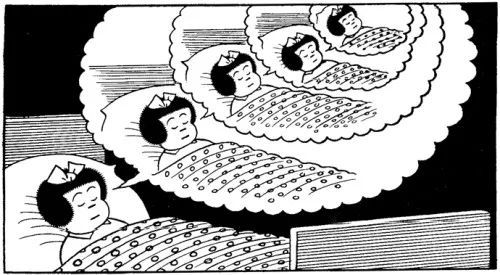
\includegraphics[scale=0.7]{img/Chapter5/5-3/1.png}
\end{figure}

\begin{figure}[H]
	\centering
	
\includegraphics[scale=0.6]{img/Chapter5/5-3/2.png}
\end{figure}

\begin{figure}[H]
	\centering
	
\includegraphics[scale=0.6]{img/Chapter5/5-3/3.png}
\end{figure}

\begin{figure}[H]
	\centering
	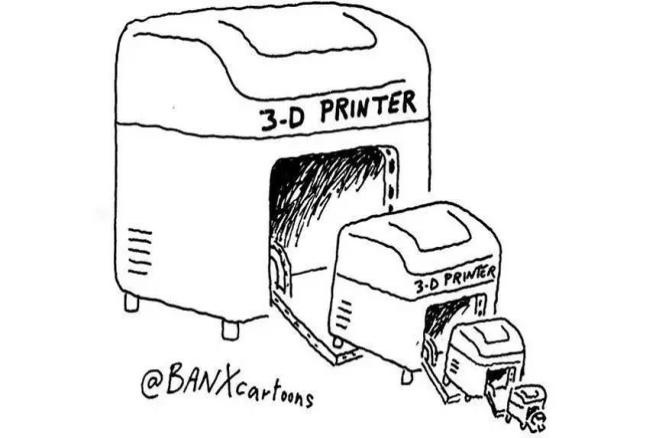
\includegraphics[scale=1.3]{img/Chapter5/5-3/4.png}
\end{figure}

\begin{figure}[H]
	\centering
	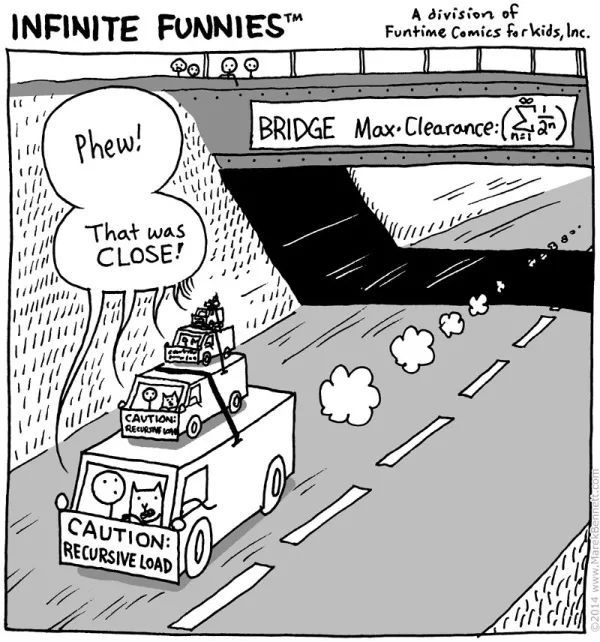
\includegraphics[scale=0.6]{img/Chapter5/5-3/5.png}
\end{figure}

\mybox{无限递归}

\begin{lstlisting}[language=C]
#include <stdio.h>

void tellStory() {
	printf("从前有座山\n");
	printf("山里有座庙\n");
	printf("庙里有个老和尚和小和尚\n");
	printf("老和尚在对小和尚讲故事\n");
	printf("他讲的故事是:\n");
	tellStory();
}

int main() {
	tellStory();
	return 0;
}
\end{lstlisting}

\begin{tcolorbox}
	\mybox{运行结果}
	\begin{verbatim}
从前有座山
山里有座庙
庙里有个老和尚和小和尚
老和尚对小和尚在讲故事
他讲的故事是:
从前有座山
山里有座庙
庙里有个老和尚和小和尚
老和尚对小和尚在讲故事
他讲的故事是:
...
	\end{verbatim}
\end{tcolorbox}

递归函数一般需要定义递归的出口,即结束条件,确保递归能够在适合的地方退出。\\

\mybox{阶乘}

\begin{lstlisting}[language=C]
#include <stdio.h>

int factorial(int n) {
    if(n == 0 || n == 1) {
        return 1;
    }
    return n * factorial(n-1);
}

int main() {
    printf("5! = %d\n", factorial(5));
    return 0;
}
\end{lstlisting}

\begin{tcolorbox}
	\mybox{运行结果}
	\begin{verbatim}
5! = 120
	\end{verbatim}
\end{tcolorbox}

\begin{figure}[H]
	\centering
	\begin{tikzpicture}[]
		\draw (0,0) rectangle (3,1.5);
		\draw (3,-2) rectangle (6,-0.5);
		\draw (6,-4) rectangle (9,-2.5);
		\draw (9,-6) rectangle (12,-4.5);
		\draw (12,-8) rectangle (15,-6.5);

		\draw (12.75,-10.75) rectangle (14.25,-9.25);
		\draw (9.75,-8.75) rectangle (11.25,-7.25);
		\draw (6.75,-6.75) rectangle (8.25,-5.25);
		\draw (3.75,-4.75) rectangle (5.25,-3.25);
		\draw (0.75,-2.75) rectangle (2.25,-1.25);

		\draw (1.5,0.75) node {$ factorial(5) $};
		\draw (4.5,-1.25) node {$ factorial(4) $};
		\draw (7.5,-3.25) node {$ factorial(3) $};
		\draw (10.5,-5.25) node {$ factorial(2) $};
		\draw (13.5,-7.25) node {$ factorial(1) $};

		\draw (13.5,-10) node {$ 1 $};
		\draw (10.5,-8) node {$ 2 $};
		\draw (7.5,-6) node {$ 6 $};
		\draw (4.5,-4) node {$ 24 $};
		\draw (1.5,-2) node {$ 120 $};

		\draw[->] (3,0.75) -- (4.5,0.75) -- (4.5,-0.5);
		\draw[->] (6,-1.25) -- (7.5,-1.25) -- (7.5,-2.5);
		\draw[->] (9,-3.25) -- (10.5,-3.25) -- (10.5,-4.5);
		\draw[->] (12,-5.25) -- (13.5,-5.25) -- (13.5,-6.5);

		\draw[->] (12.75,-10) -- (10.5,-10) -- (10.5,-8.75);
		\draw[->] (9.75,-8) -- (7.5,-8) -- (7.5,-6.75);
		\draw[->] (6.75,-6) -- (4.5,-6) -- (4.5,-4.75);
		\draw[->] (3.75,-4) -- (1.5,-4) -- (1.5,-2.75);

		\draw (4.5,1) node {$ 5 * factorial(4) $};
		\draw (7.5,-1) node {$ 4 * factorial(3) $};
		\draw (10.5,-3) node {$ 3 * factorial(2) $};
		\draw (13.5,-5) node {$ 2 * factorial(1) $};

		\draw (11,-10.5) node {$ 2 * 1 $};
		\draw (8,-8.5) node {$ 3 * 2 $};
		\draw (5,-6.5) node {$ 4 * 6 $};
		\draw (2,-4.5) node {$ 5 * 24 $};
	\end{tikzpicture}
	\caption{阶乘}
\end{figure}

\mybox{斐波那契数列(递归)}

\begin{lstlisting}[language=C]
#include <stdio.h>

int fibonacci(int n) {
    if(n == 1 || n == 2) {
        return 1;
    }
    return fibonacci(n-2) + fibonacci(n-1);
}

int main() {
    int n = 7;
    printf("斐波那契数列第%d位:%d\n", n, fibonacci(n));
    return 0;
}
\end{lstlisting}

\begin{tcolorbox}
	\mybox{运行结果}
	\begin{verbatim}
斐波那契数列第7位:13
	\end{verbatim}
\end{tcolorbox}

\begin{figure}[H]
	\centering
	\begin{tikzpicture}[
			level distance=2.4cm,
			level 1/.style={sibling distance=6cm},
			level 2/.style={sibling distance=3cm},
			level 3/.style={sibling distance=2cm}
		]
		\node {$ f(5) $}
		child {
				node {$ f(3) $}
				child {node {$ f(1) $}}
				child {
						node {$ f(2) $}
						child {node {$ f(0) $}}
						child {node {$ f(1) $}}
					}
			}
		child {
				node {$ f(4) $}
				child {
						node {$ f(2) $}
						child {node {$ f(0) $}}
						child {node {$ f(1) $}}
					}
				child {
						node {$ f(3) $}
						child {node {$ f(1) $}}
						child {
								node {$ f(2) $}
								child {node {$ f(0) $}}
								child {node {$ f(1) $}}
							}
					}
			};
	\end{tikzpicture}
	\caption{递归树}
\end{figure}

\mybox{斐波那契数列(迭代)}

\begin{lstlisting}[language=C]
#include <stdio.h>

int fibonacci(int n) {
    int f[n];
    f[0] = f[1] = 1;
    for(int i = 2; i < n; i++) {
        f[i] = f[i-2] + f[i-1];
    }
    return f[n-1];
}

int main() {
    int n = 7;
    printf("斐波那契数列第%d位:%d\n", n, fibonacci(n));
    return 0;
}
\end{lstlisting}

\begin{tcolorbox}
	\mybox{运行结果}
	\begin{verbatim}
斐波那契数列第7位:13
	\end{verbatim}
\end{tcolorbox}

\vspace{0.5cm}

\mybox{阿克曼函数}

\begin{align}\nonumber
	A(m, n) =
	\begin{cases}
		n + 1             & m = 0        \\
		A(m-1, 1)         & m > 0, n = 0 \\
		A(m-1, A(m, n-1)) & m > 0, n > 0 \\
	\end{cases}
\end{align}

\begin{lstlisting}[language=C]
#include <stdio.h>

int A(int m, int n) {
    if(m == 0) {
        return n + 1;
    } else if(m > 0 && n == 0) {
        return A(m-1, 1);
    } else {
        return A(m-1, A(m, n-1));
    }
}

int main() {
    printf("%d\n", A(3, 4));
    return 0;
}
\end{lstlisting}

\begin{tcolorbox}
	\mybox{运行结果}
	\begin{verbatim}
125
	\end{verbatim}
\end{tcolorbox}

\begin{table}[H]
	\centering
	\setlength{\tabcolsep}{0.5mm}{
		\begin{tabular}{|c|c|c|c|c|c|c|}
			\hline
			\diagbox{$ m $}{$ n $} & \textbf{$ 0 $} & \textbf{$ 1 $}    & \textbf{$ 2 $}    & \textbf{$ 3 $}          & \textbf{$ 4 $}    & \textbf{$ n $}                                         \\
			\hline
			\textbf{$ 0 $}         & $ 1 $          & $ 2 $             & $ 3 $             & $ 4 $                   & $ 5 $             & $ n + 1 $                                              \\
			\hline
			\textbf{$ 1 $}         & $ 2 $          & $ 3 $             & $ 4 $             & $ 5 $                   & $ 6 $             & $ 2 + (n + 3) - 3 $                                    \\
			\hline
			\textbf{$ 2 $}         & $ 3 $          & $ 5 $             & $ 7 $             & $ 9 $                   & $ 11 $            & $ 2(n + 3) - 3 $                                       \\
			\hline
			\textbf{$ 3 $}         & $ 5 $          & $ 13 $            & $ 29 $            & $ 61 $                  & $ 125 $           & $ 2^{n + 3} - 3 $                                      \\
			\hline
			\textbf{$ 4 $}         & $ 13 $         & $ 65533 $         & $ 2^{65536} - 3 $ & $ A(3, 2^{65536} - 3) $ & $ A(3, A(4, 3)) $ & $ \underbrace{2^{2^{.^{.^{.{^2}}}}}}_{n+3\ twos} - 3 $ \\
			\hline
			\textbf{$ 5 $}         & $ 65533 $      & $ A(4, 65533) $   & $ A(4, A(5, 1)) $ & $ A(4, A(5, 2)) $       & $ A(4, A(5, 3)) $ & $ \dots $                                              \\
			\hline
			\textbf{$ 6 $}         & $ A(5, 1) $    & $ A(5, A(5, 1)) $ & $ A(5, A(6, 1)) $ & $ A(5, A(6, 2)) $       & $ A(5, A(6, 3)) $ & $ \dots $                                              \\
			\hline
		\end{tabular}
	}
	\caption{阿克曼函数}
\end{table}

\begin{figure}[H]
	\centering
	
\includegraphics[]{img/Chapter5/5-3/6.png}
\end{figure}

\mybox{汉诺塔}\\

给定三根柱子,其中A柱子从大到小套有n个圆盘,问题是如何借助B柱子,将圆盘从A搬到C。\\

规则:

\begin{itemize}
	\item 一次只能搬动一个圆盘
	\item 不能将大圆盘放在小圆盘上面
\end{itemize}

\begin{figure}[H]
	\centering
	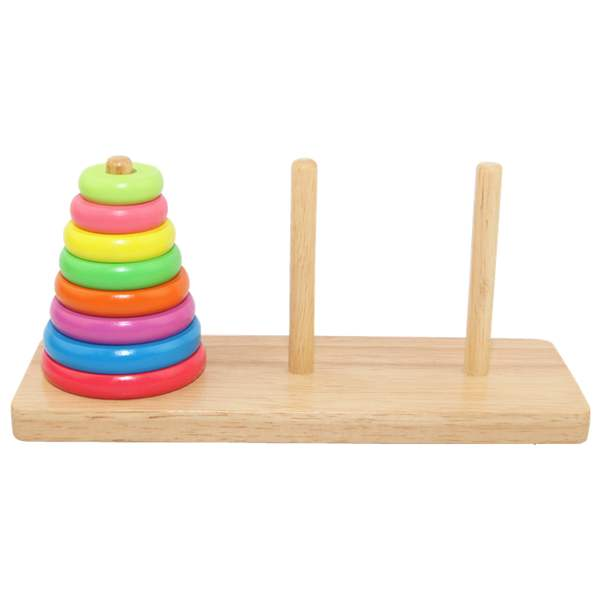
\includegraphics[scale=0.4]{img/Chapter5/5-3/7.png}
\end{figure}

递归算法求解汉诺塔问题:

\begin{enumerate}
	\item 将前n-1个圆盘从A柱借助于C柱搬到B柱。
	\item 将最后一个圆盘直接从A柱搬到C柱。
	\item 将n-1个圆盘从B柱借助于A柱搬到C柱。
\end{enumerate}

\begin{lstlisting}[language=C]
#include <stdio.h>

int move = 0;       // 移动次数

/**
    * @brief  汉诺塔算法
    * @note   把 n 个盘子从 src 借助 mid 移到 dst
    * @param  n: 层数
    * @param  src: 起点柱子
    * @param  mid: 临时柱子
    * @param  dst: 目标柱子
    */
void hanoi(int n, char src, char mid, char dst) {
    if(n == 1) {
        printf("%d号盘:%c -> %c\n", n, src, dst);
        move++;
    } else {
        // 把前 n-1 个盘子从 src 借助 dst 移到 mid
        hanoi(n-1, src, dst, mid);
        // 移动第 n 个盘子
        printf("%d号盘:%c -> %c\n", n, src, dst);
        move++;
        // 把刚才的 n-1 个盘子从 mid 借助 src 移到 dst
        hanoi(n-1, mid, src, dst);
    }
}

int main() {
    hanoi(4, 'A', 'B', 'C');
    printf("步数 ==> %d\n", move);
    return 0;
}
\end{lstlisting}

\begin{tcolorbox}
	\mybox{运行结果}
	\begin{verbatim}
1号盘:A -> B
2号盘:A -> C
1号盘:B -> C
3号盘:A -> B
1号盘:C -> A
2号盘:C -> B
1号盘:A -> B
4号盘:A -> C
1号盘:B -> C
2号盘:B -> A
1号盘:C -> A
3号盘:B -> C
1号盘:A -> B
2号盘:A -> C
1号盘:B -> C
步数 ==> 15
	\end{verbatim}
\end{tcolorbox}

\newpage